\graphicspath{
  {./images/bmps/}{./images/vects/}{./images/}
  {./images/presentation/bmps/}{./images/presentation/vects/}{./images/presentation/}
  {./images/chapter00/bmps/}{./images/chapter00/vects/}{./images/chapter00/}
  {./images/chapter06/bmps/}{./images/chapter06/vects/}{./images/chapter06/}
  {./images/chapter07/bmps/}{./images/chapter07/vects/}{./images/chapter07/}
}

\begin{frame}
  \frametitle{Table of Contents}
  \tiny
  \tableofcontents[currentsection]
\end{frame}
  
\begin{frame}{Planning}
  \begin{columns}[c] % the "c" option specifies center vertical alignment
    \column{.5\textwidth} % column designated by a command
      \begin{overlayarea}{\textwidth}{\textheight}
	\begin{itemize}
	\item Global Planner
	\end{itemize}
	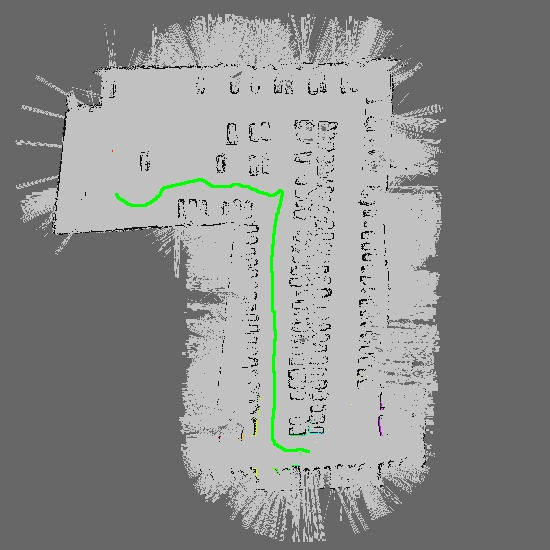
\includegraphics[width=\textwidth]{figure7}
      \end{overlayarea}
    \column{.5\textwidth}
      \begin{overlayarea}{\textwidth}{\textheight}
	\begin{itemize}
	\item Local Planner
	\end{itemize}
	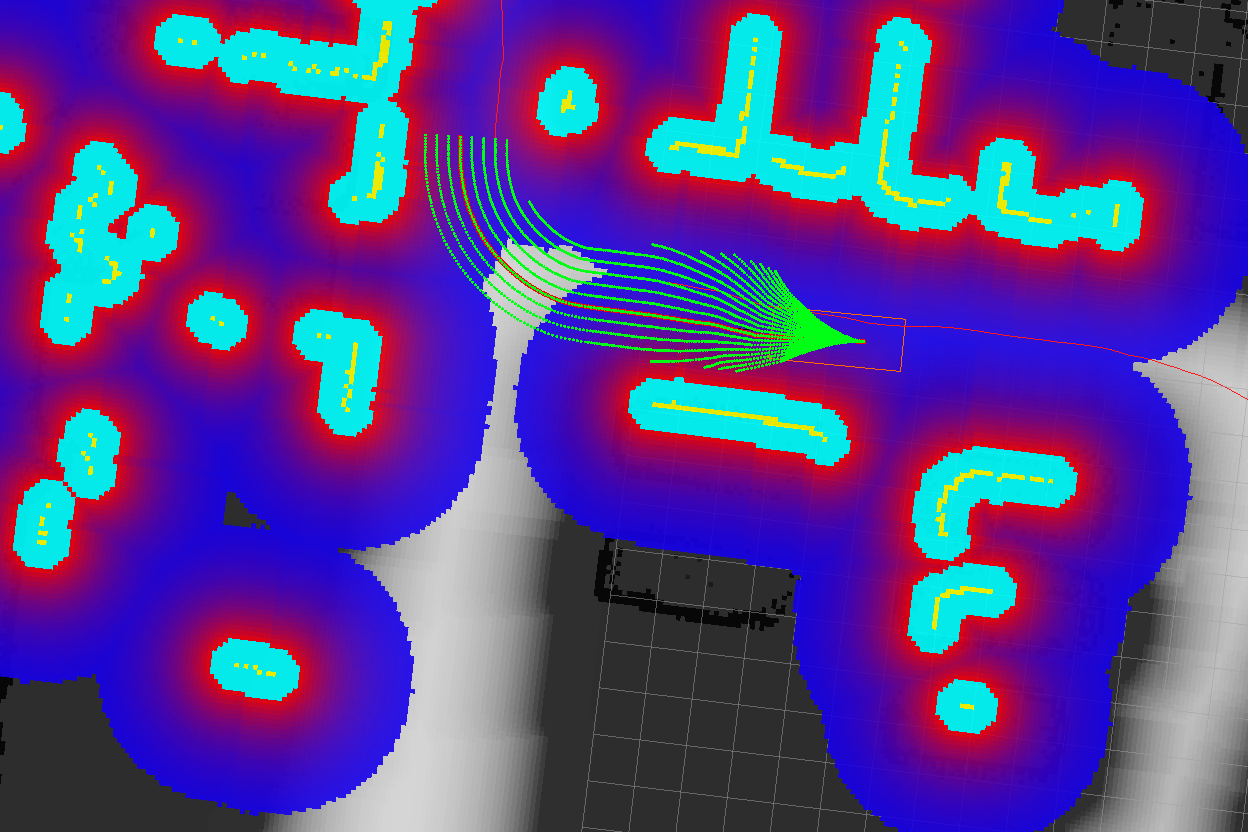
\includegraphics[width=\textwidth]{example14}
	\end{overlayarea}
  \end{columns}
\end{frame}

\subsection{Global Planning}

\begin{frame}{Introduction}
  \begin{itemize}
   \item Based on a Multiclass Support Vector Machine (MSVM)
   \item Advantages:
   \begin{enumerate}
    \item Smooth paths (Non-linear hyperplanes).
    \item Safe paths (Margin maximization).
    \item Noise tolerance (Margin maximization).
    \item Automatic generation of a RNDF (MSVM).
   \end{enumerate}
  \end{itemize}
  \begin{center}
    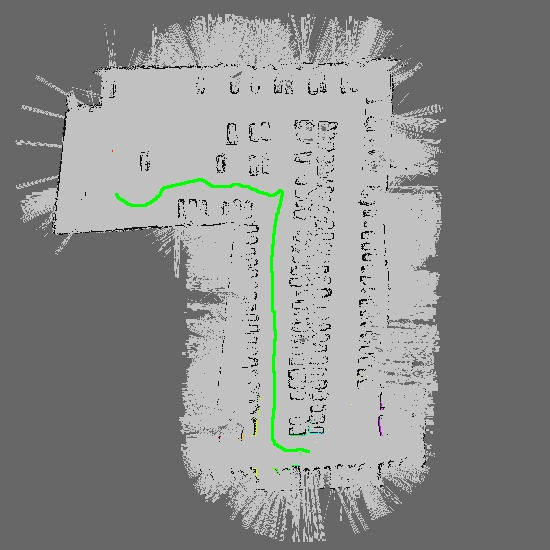
\includegraphics[height=0.4\textheight]{figure7}
  \end{center}
  
  \note {
  Advantages:
   \begin{enumerate}
      \item With SVM, it is possible to generate non-linear hyperplanes which limit areas in the ground, allowing the generation of smooth paths.
      \item Margin maximization allows performing a safe search strategy, ensuring that the path will always be at a certain distance the obstacles.
      \item By using SVM, the uncertainty due to the errors introduced by sensors is reduced, since they try to maximize the distance to the points that define different obstacles. If it is not possible to define a line that clearly divides two different regions, a function that tries to minimize this effect is generated.
      \item In addition to these features, the use of MSVM adds another advantage.  By using them, \emph{all} possible routes in a map can be generated ensuring that they will be safe (the distance to the obstacles will be optimal) and smooth.
   \end{enumerate}
  }

\end{frame}

\begin{frame}[plain]{Pipeline}
  \begin{center}
    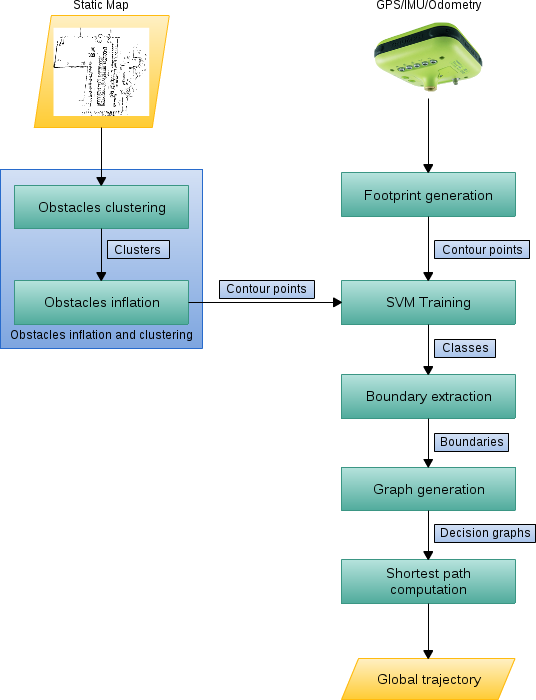
\includegraphics[height=1.1\textheight]{pipeline_cp06}
  \end{center}
  \note{
  }
\end{frame}

\begin{frame}{Costmap generation}
   \begin{center}
    \begin{equation}\nonumber
      \mathcal{C}(i, j) = \exp (-1.0 \cdot \alpha \cdot ( \|c_{ij}-\vec{o}\| - \rho_{inscribed})) \cdot 253
    \end{equation}\\~\\
    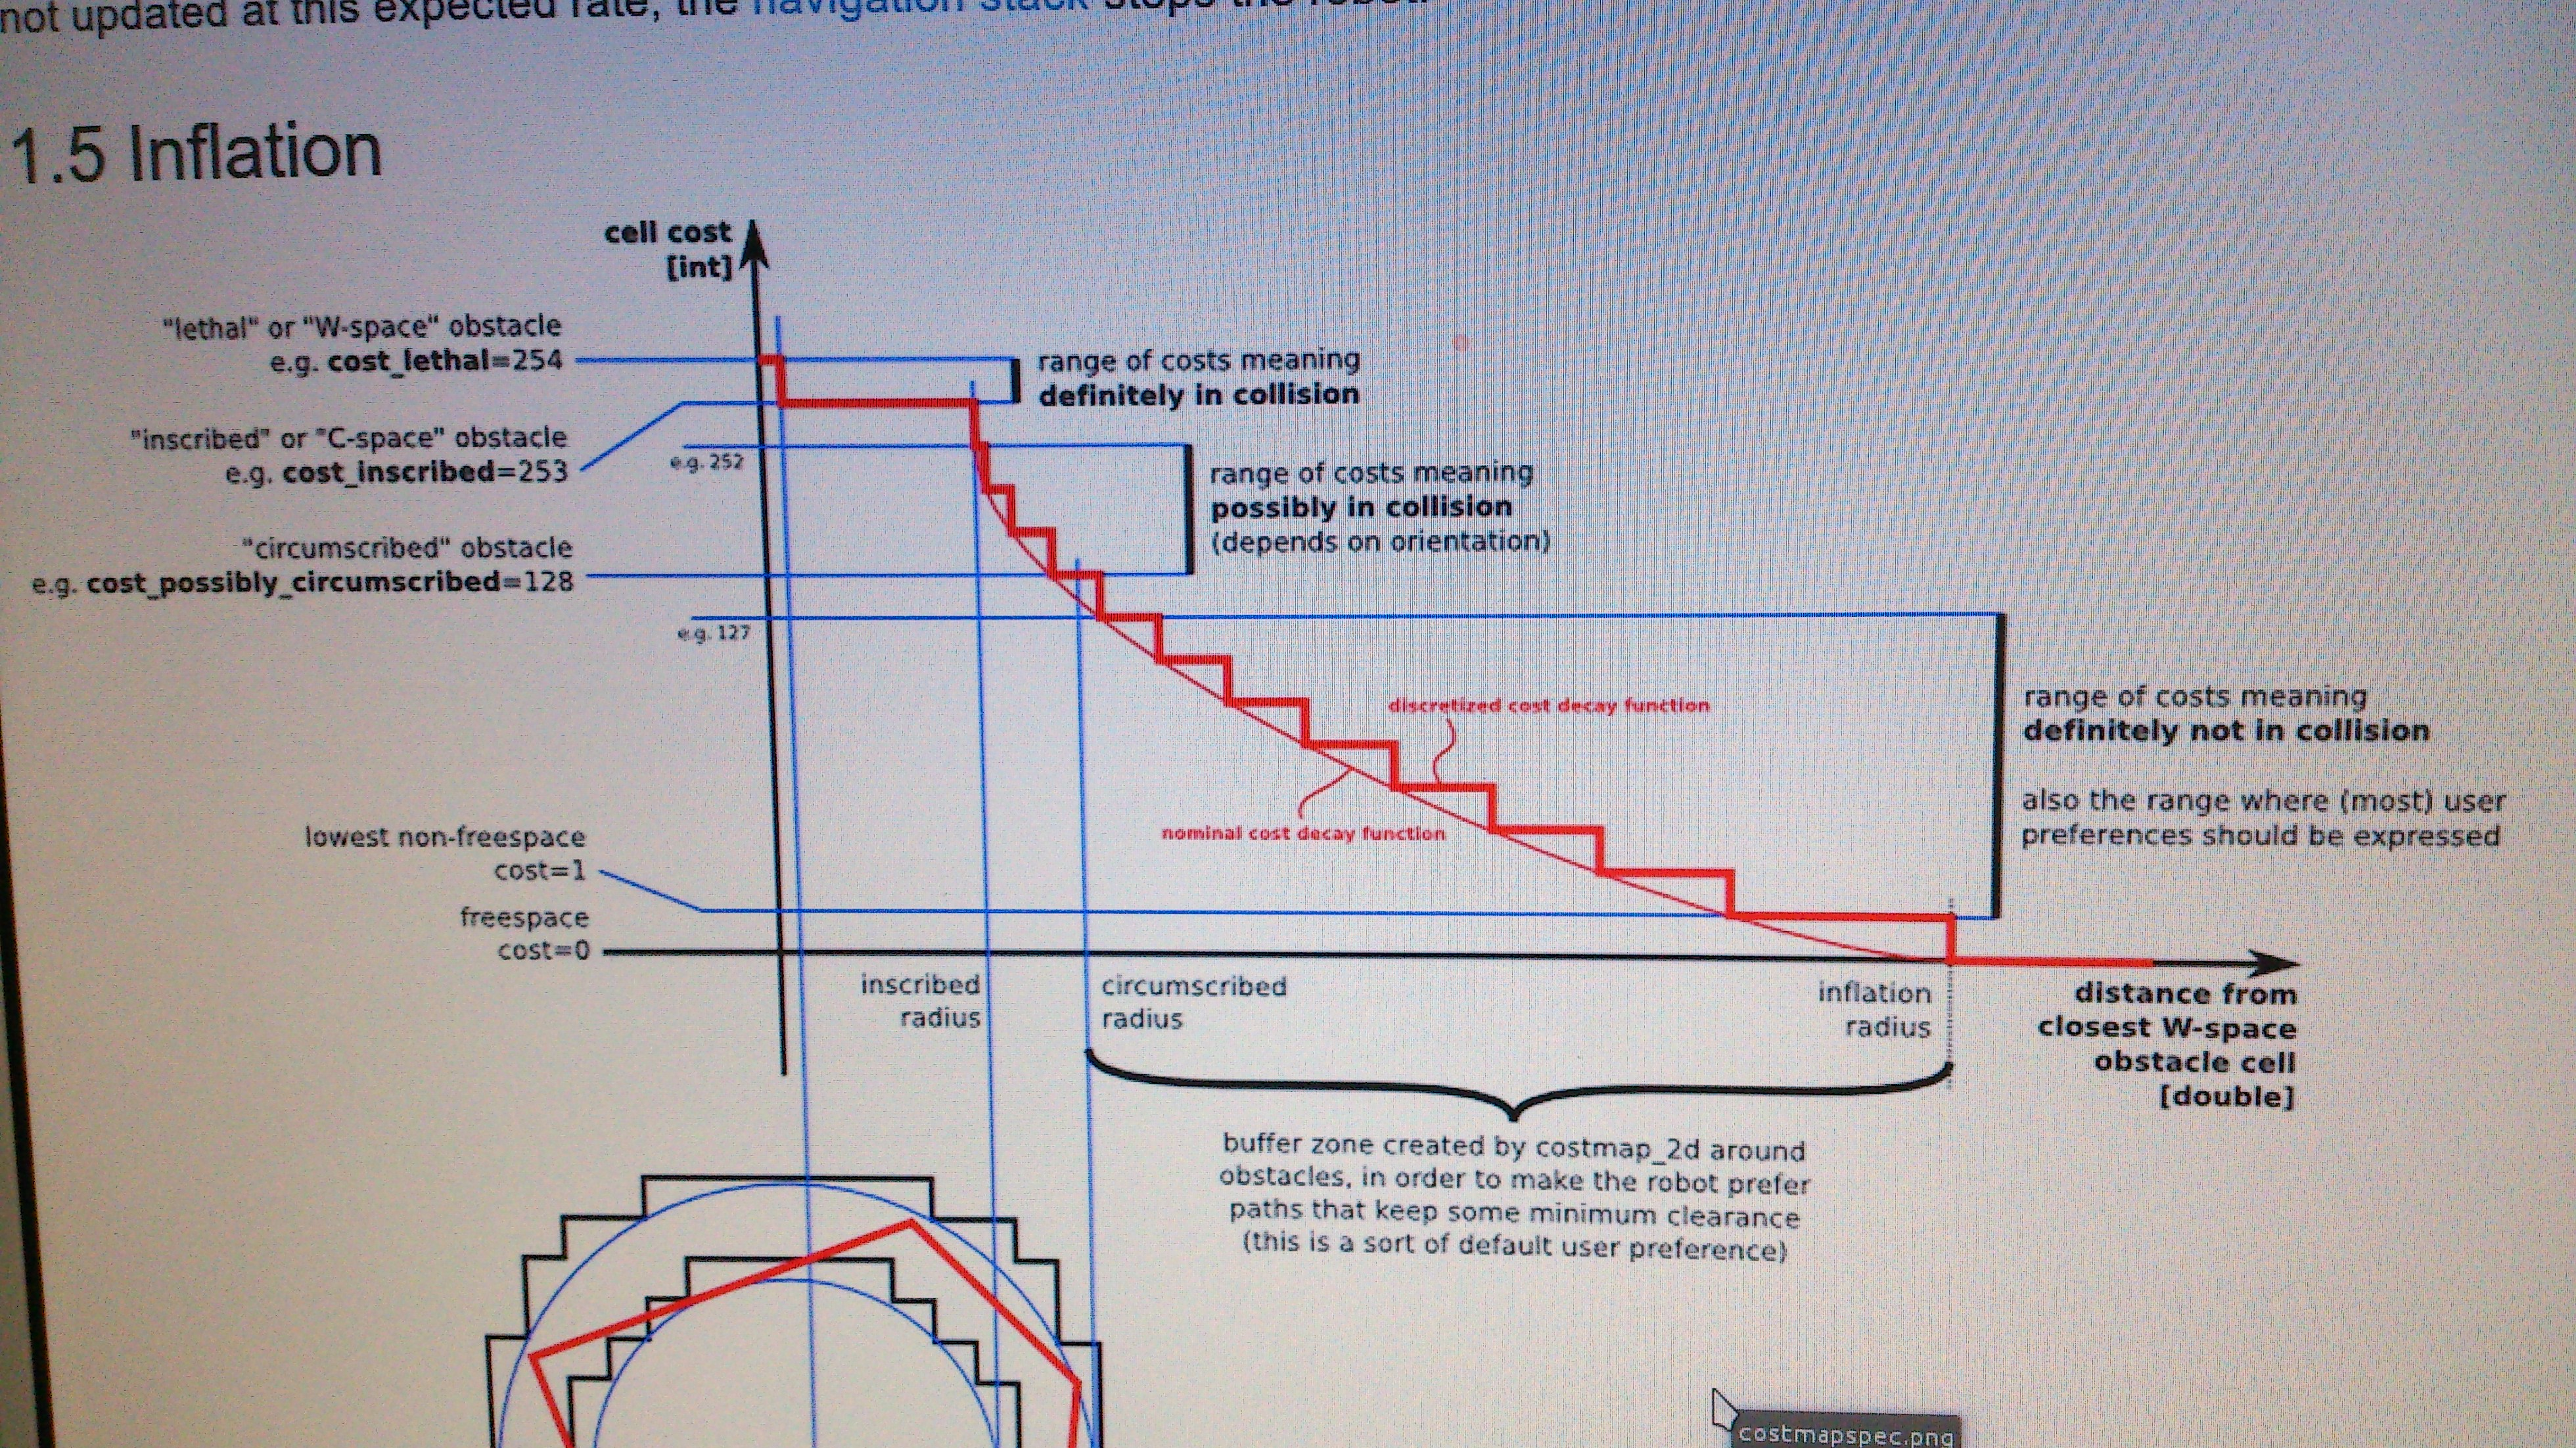
\includegraphics[height=0.5\textheight]{cost_levels}
    ~
    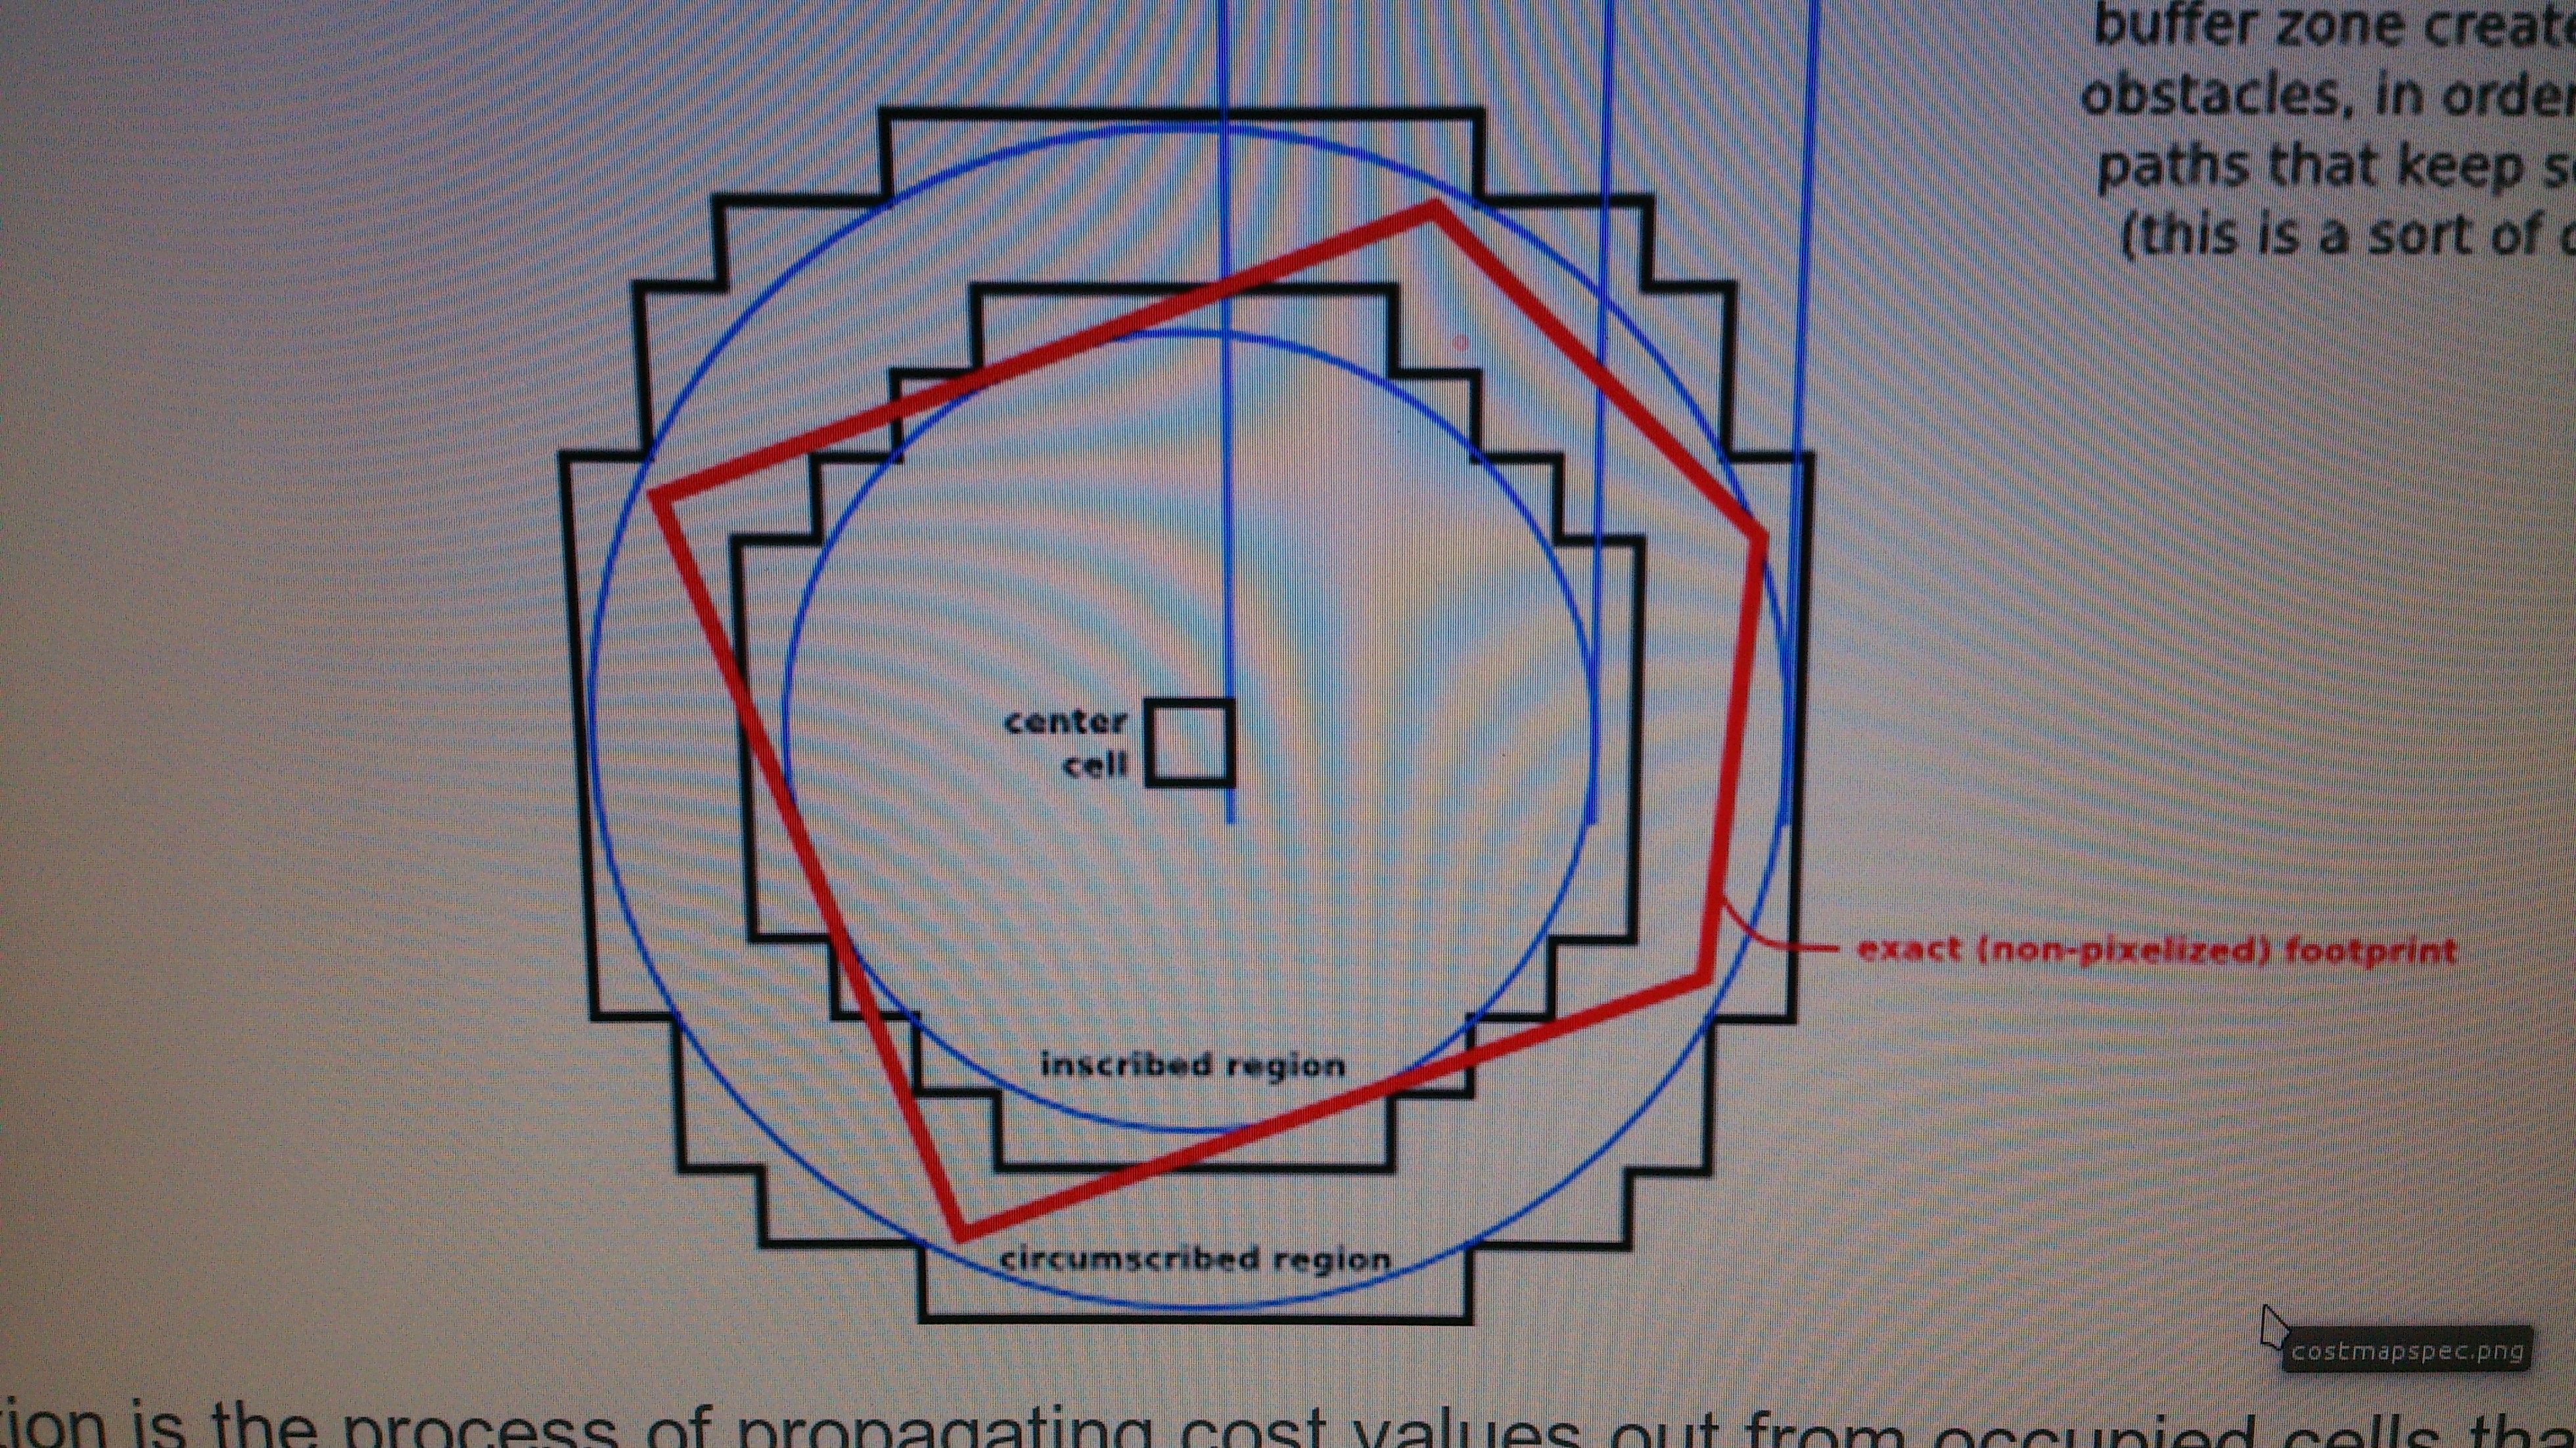
\includegraphics[height=0.5\textheight]{inscribed_circumscribed}
  \end{center}
  
  \note {

  }
\end{frame}

\begin{frame}{First execution}
  \begin{columns}
  \column{0.4\textwidth}
    \hskip -0.5cm
    \begin{overlayarea}{\textwidth}{\textheight}
      \begin{enumerate}
	\item<1-> Obstacles inflation.
	\item<1-> Obstacles clustering.
	\item<3-> SVM training.
	\item<4-> Boundary extraction.
	\item<5-> Graph generation.
      \end{enumerate}
    \end{overlayarea}
  \column{0.69\textwidth}
    \vskip -1cm
    \begin{overlayarea}{\textwidth}{\textheight}
      \only<1> {
	\begin{block}{Obstacles inflation}
	  \begin{itemize}
	    \item World map is represented as a grid of a certain resolution.
	    \item Costmap is binarized and boundaries extracted\footnote{\cite{suzuki1985topological}}.
	    \item Boundaries are clustered\footnote{\cite{rusu2009semantic}}
	  \end{itemize}
	\end{block}
      }
      \only<2> {
	\vskip 0.25cm
	\begin{figure}	
	  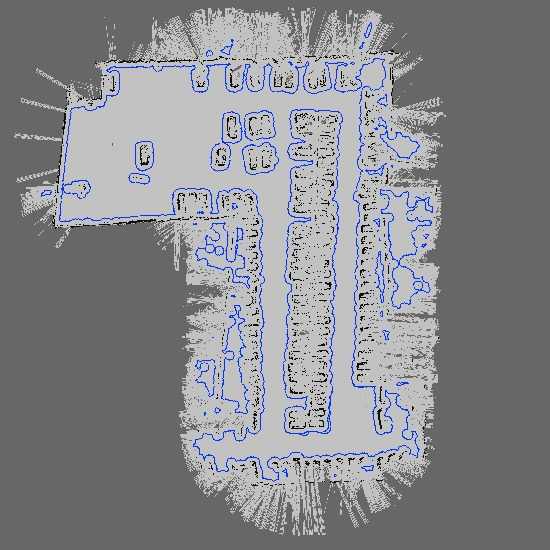
\includegraphics[height=0.7\textheight]{figure1}
	\end{figure}
      }
      \only<3> {
	\begin{block}{SVM training}
	  \begin{itemize}
	    \item One-versus-all strategy.
	    \item For each SVM $k$
	    \begin{itemize}
	      \item Parameters $\alpha_k ~ \rightarrow$  support vectors $x_k$.
	      \item Labels $y_k$.
	    \end{itemize}
	    \item GPU implementation of the SVM\footnote{\cite{athanasopoulos2011gpu}}.
	  \end{itemize}
	\end{block}
      }
    \only<4> {
	\begin{block}{}
	\footnotesize
	  \begin{itemize}
	    \item We look for the points ($x$) satisfying:
	    \begin{figure}
	      $y = \sum \limits_{k \in S} \alpha_k \cdot y_k \cdot  K(x_k, x) + b = 0$
	      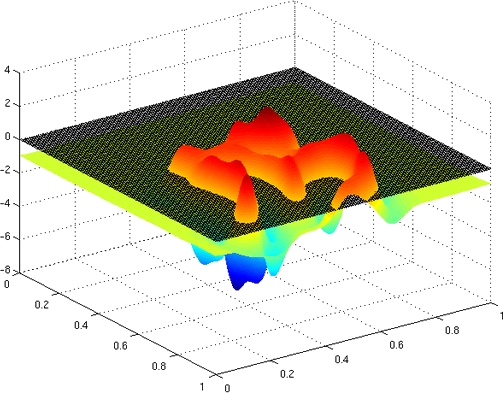
\includegraphics[height=0.4\textheight]{figure2}
	    \end{figure}
	    \item Map is sampled on a grid.
	    \item $y$ is computed for each cell using the GPU.
	    \item Decision boundaries are extracted.
	  \end{itemize}
	\end{block}
      }
     \only<5-7> {
	\begin{block}{Graph generation}
	\footnotesize
	  \begin{itemize}
	    \item Generation of a connectivity graph.
	    \begin{itemize}
	     \item<5-> Nearest-Neighbor Graph (NNG)
	     \item<6-> Relative Neighborhood Graph (RNG)
	    \end{itemize}
	    \item<7-> Over the GPU.
	  \end{itemize}
	  
	  \only<5> {
	    \vskip-0.5cm
	    \begin{figure}
	      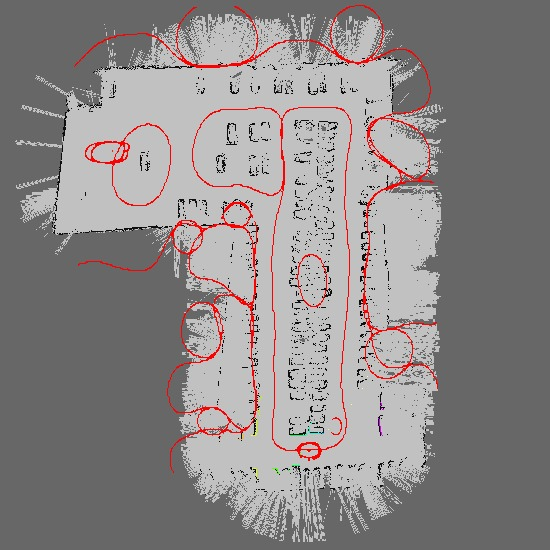
\includegraphics[height=0.5\textheight]{figure3}
	    \end{figure}
	  }
	  \only<6-7> {
	    \vskip-0.5cm
	    \begin{figure}
	      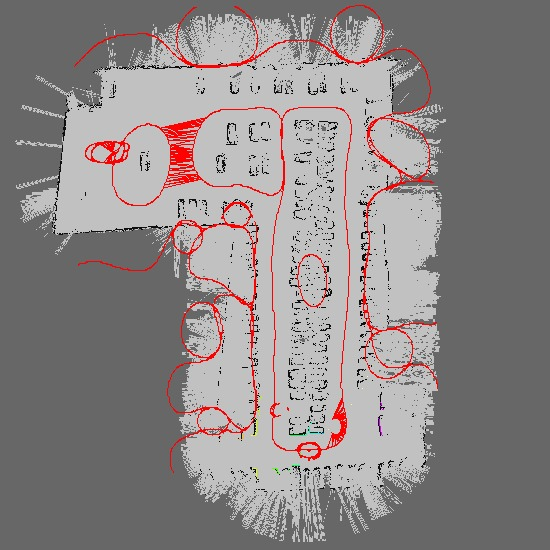
\includegraphics[height=0.5\textheight]{figure4}
	    \end{figure}	     
	  }
	\end{block}
      }
    \end{overlayarea}
  \end{columns}

  \note{
  \begin{itemize}
   \item $\beta$ is a scaling factor that increases/decreases the slope of the cost function, $nearest(c)$ is the position of the nearest cell in the map to the cell $c$ marked as obstacle, and $\rho$ is the circumscribed radius of the robot. The function is scaled to $253$ as 254 and 255 are reserved values.
   \item Onve-versus-all: for each set of points $C_i$ corresponding to a cluster in the set of clusters $\mathcal{C}$, we create two classes, one formed by the point set $C_i$, and the other composed by the points belonging to the remaining clusters $\{\mathcal{C} - C_i\}$. From these two classes, we train a single SVM, which will give us the parameters $\alpha_k$ corresponding to the support vectors $x_k$ and their labels $y_k$
   For the generation of the RNG, we use the set of labels $l_i \in \mathcal{L}$. First, we obtain the Delaunay Triangulation using the points in $\mathcal{B}$ as input. 
   \item Then, we iterate through the edges $e(u,v)$ of the triangles. For each one of these edges, we check that there are not obstacles between $u$ and $v$. If this condition is true, and $l_u \neq l_v$, the edge $e$ is added to our graph.   
  \end{itemize}

  }
\end{frame}

% \begin{frame}{Successive executions}
%   \begin{columns}
%   \hskip -0.5cm
%   \column{0.4\textwidth}
%     \begin{overlayarea}{\textwidth}{\textheight}
%       \begin{enumerate}
% 	\item<1-> Obstacles inflation and clustering.
% 	\item<2-> Footprint generation.
% 	\item<3-> SVM training and graph generation.
% 	\item<4-> Shortest path calculation.
%       \end{enumerate}
%     \end{overlayarea}
%   \column{0.69\textwidth}
%     \vskip -1cm
%     \begin{overlayarea}{\textwidth}{\textheight}
%       \only<1> {
% 	\begin{block}{Obstacles inflation and clustering}
% 	  \begin{itemize}
% 	    \item Step similar to the first iteration.
% 	    \item Using a \emph{kd-tree}, we look for differences.
% 	  \end{itemize}
% 	\end{block}
%       }
%       \only<2> {
% 	\begin{block}{Footprint generation}
% 	  \begin{figure}
% 	      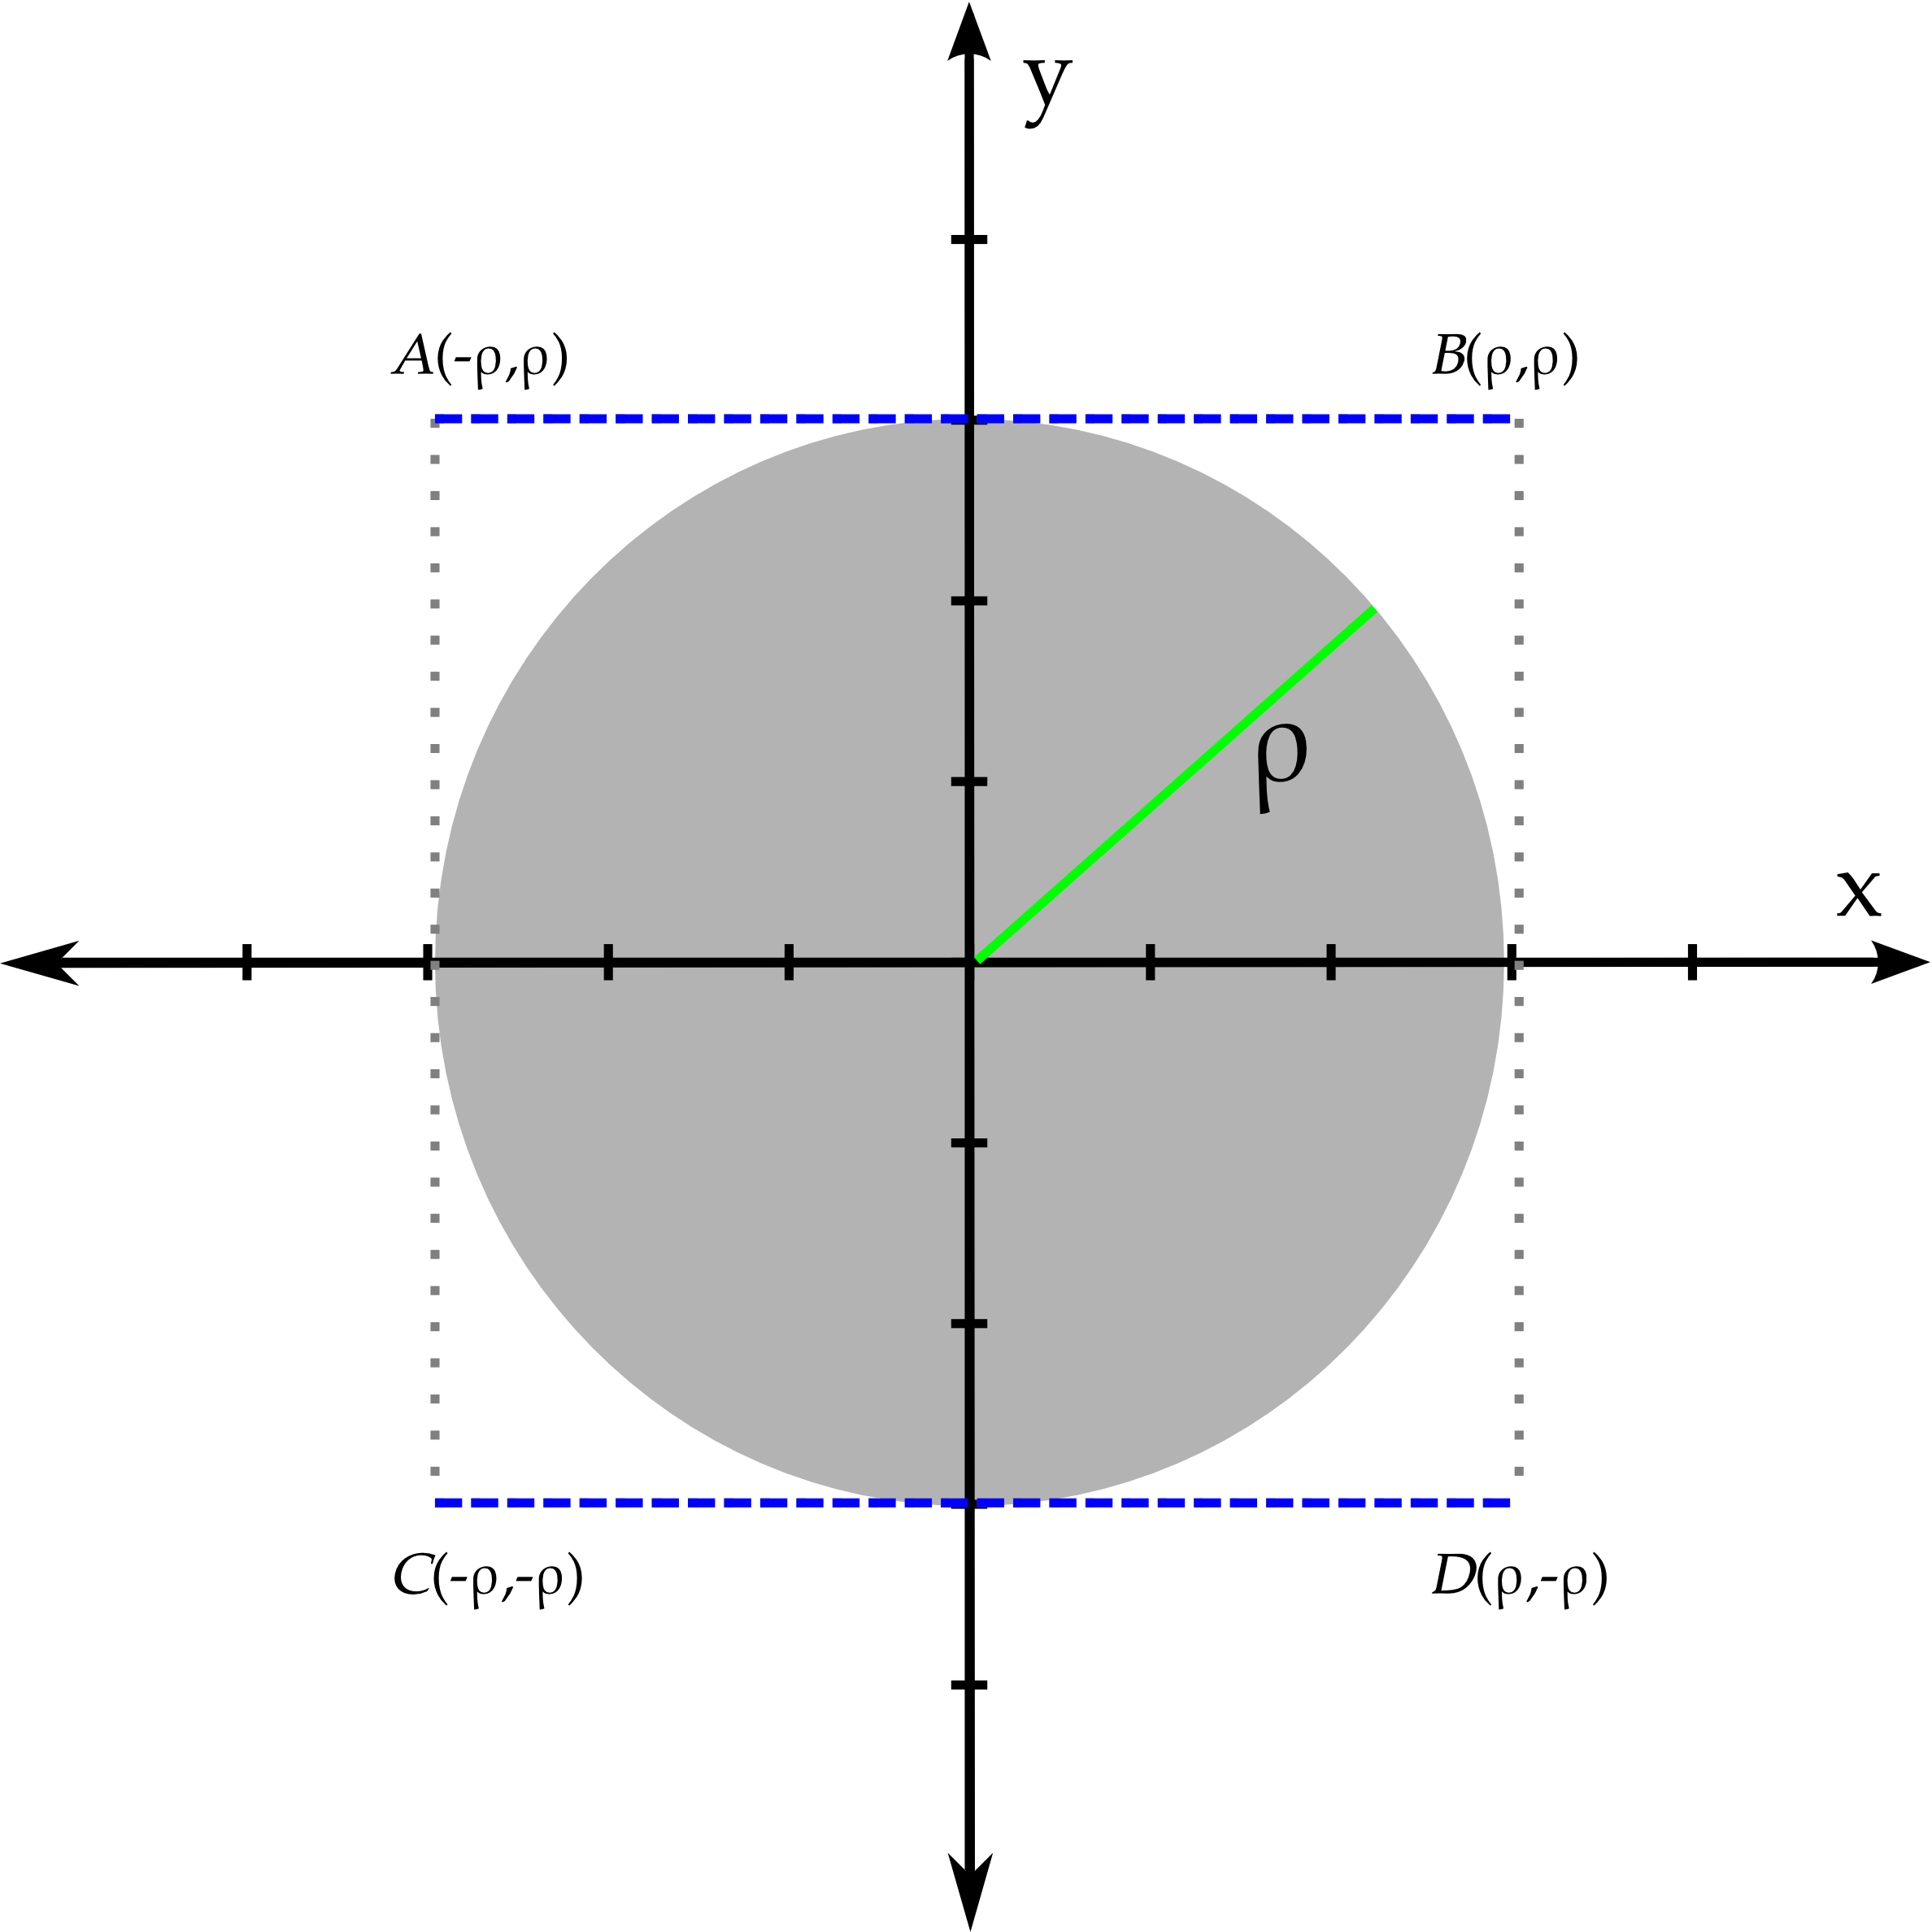
\includegraphics[height=0.4\textheight]{figure5}
% 	  \end{figure}
% 	  \vskip-0.65cm
% 	  \begin{itemize}
% 	    \item Footprint is transformed to map coordinates
% 	  \end{itemize}
% 	  \begin{equation}
% 	    \footnotesize \nonumber
% 	    Rt = \left ( \begin{array}{ ccc }
% 	      \cos(\theta_s) & -\sin(\theta_s) & s_x \\
% 	      \cos(\theta_s) & -\sin(\theta_s) & s_y \\
% 	      0 & 0 & 1
% 	    \end{array} \right )
% 	  \end{equation}
% 	\end{block}
%       }
%       \only<3> {
% 	\begin{block}{SVM training and graph generation}
% 	  \begin{itemize}
% 	    \item Similar to first execution.
% 	    \item Differences:
% 	    \begin{itemize}
% 	     \item No traversable paths are removed.
% 	     \item New traversable paths are added.
% 	    \end{itemize}
% 	  \end{itemize}
% 	\end{block}
%       }
%       \only<4-5> {
% 	\only<4-> {
% 	  \begin{block}{Looking for starting and goal points}
% 	    \only<4> {
% 	      \begin{itemize}
% 		\item Sense is restricted by using $s_1$ and $g_1$.
% 		  \begin{equation}\nonumber
% 		  \footnotesize
% 		  \begin {array}{l}
% 		  s_1 = (s_x + \rho * \cos(\theta_s), s_y + \rho * \sin(\theta_s)) \\
% 		  g_1 = (g_x - \rho * \cos(\theta_g), g_y - \rho * \sin(\theta_g))
% 		  \end{array}
% 		  \end{equation}
% 		\item A \emph{kd-tree} is used to find the nearest point in the graph.
% 	      \end{itemize}
% 	      \vskip-0.5cm
% 	    }
% 	    \begin{figure}
% 	      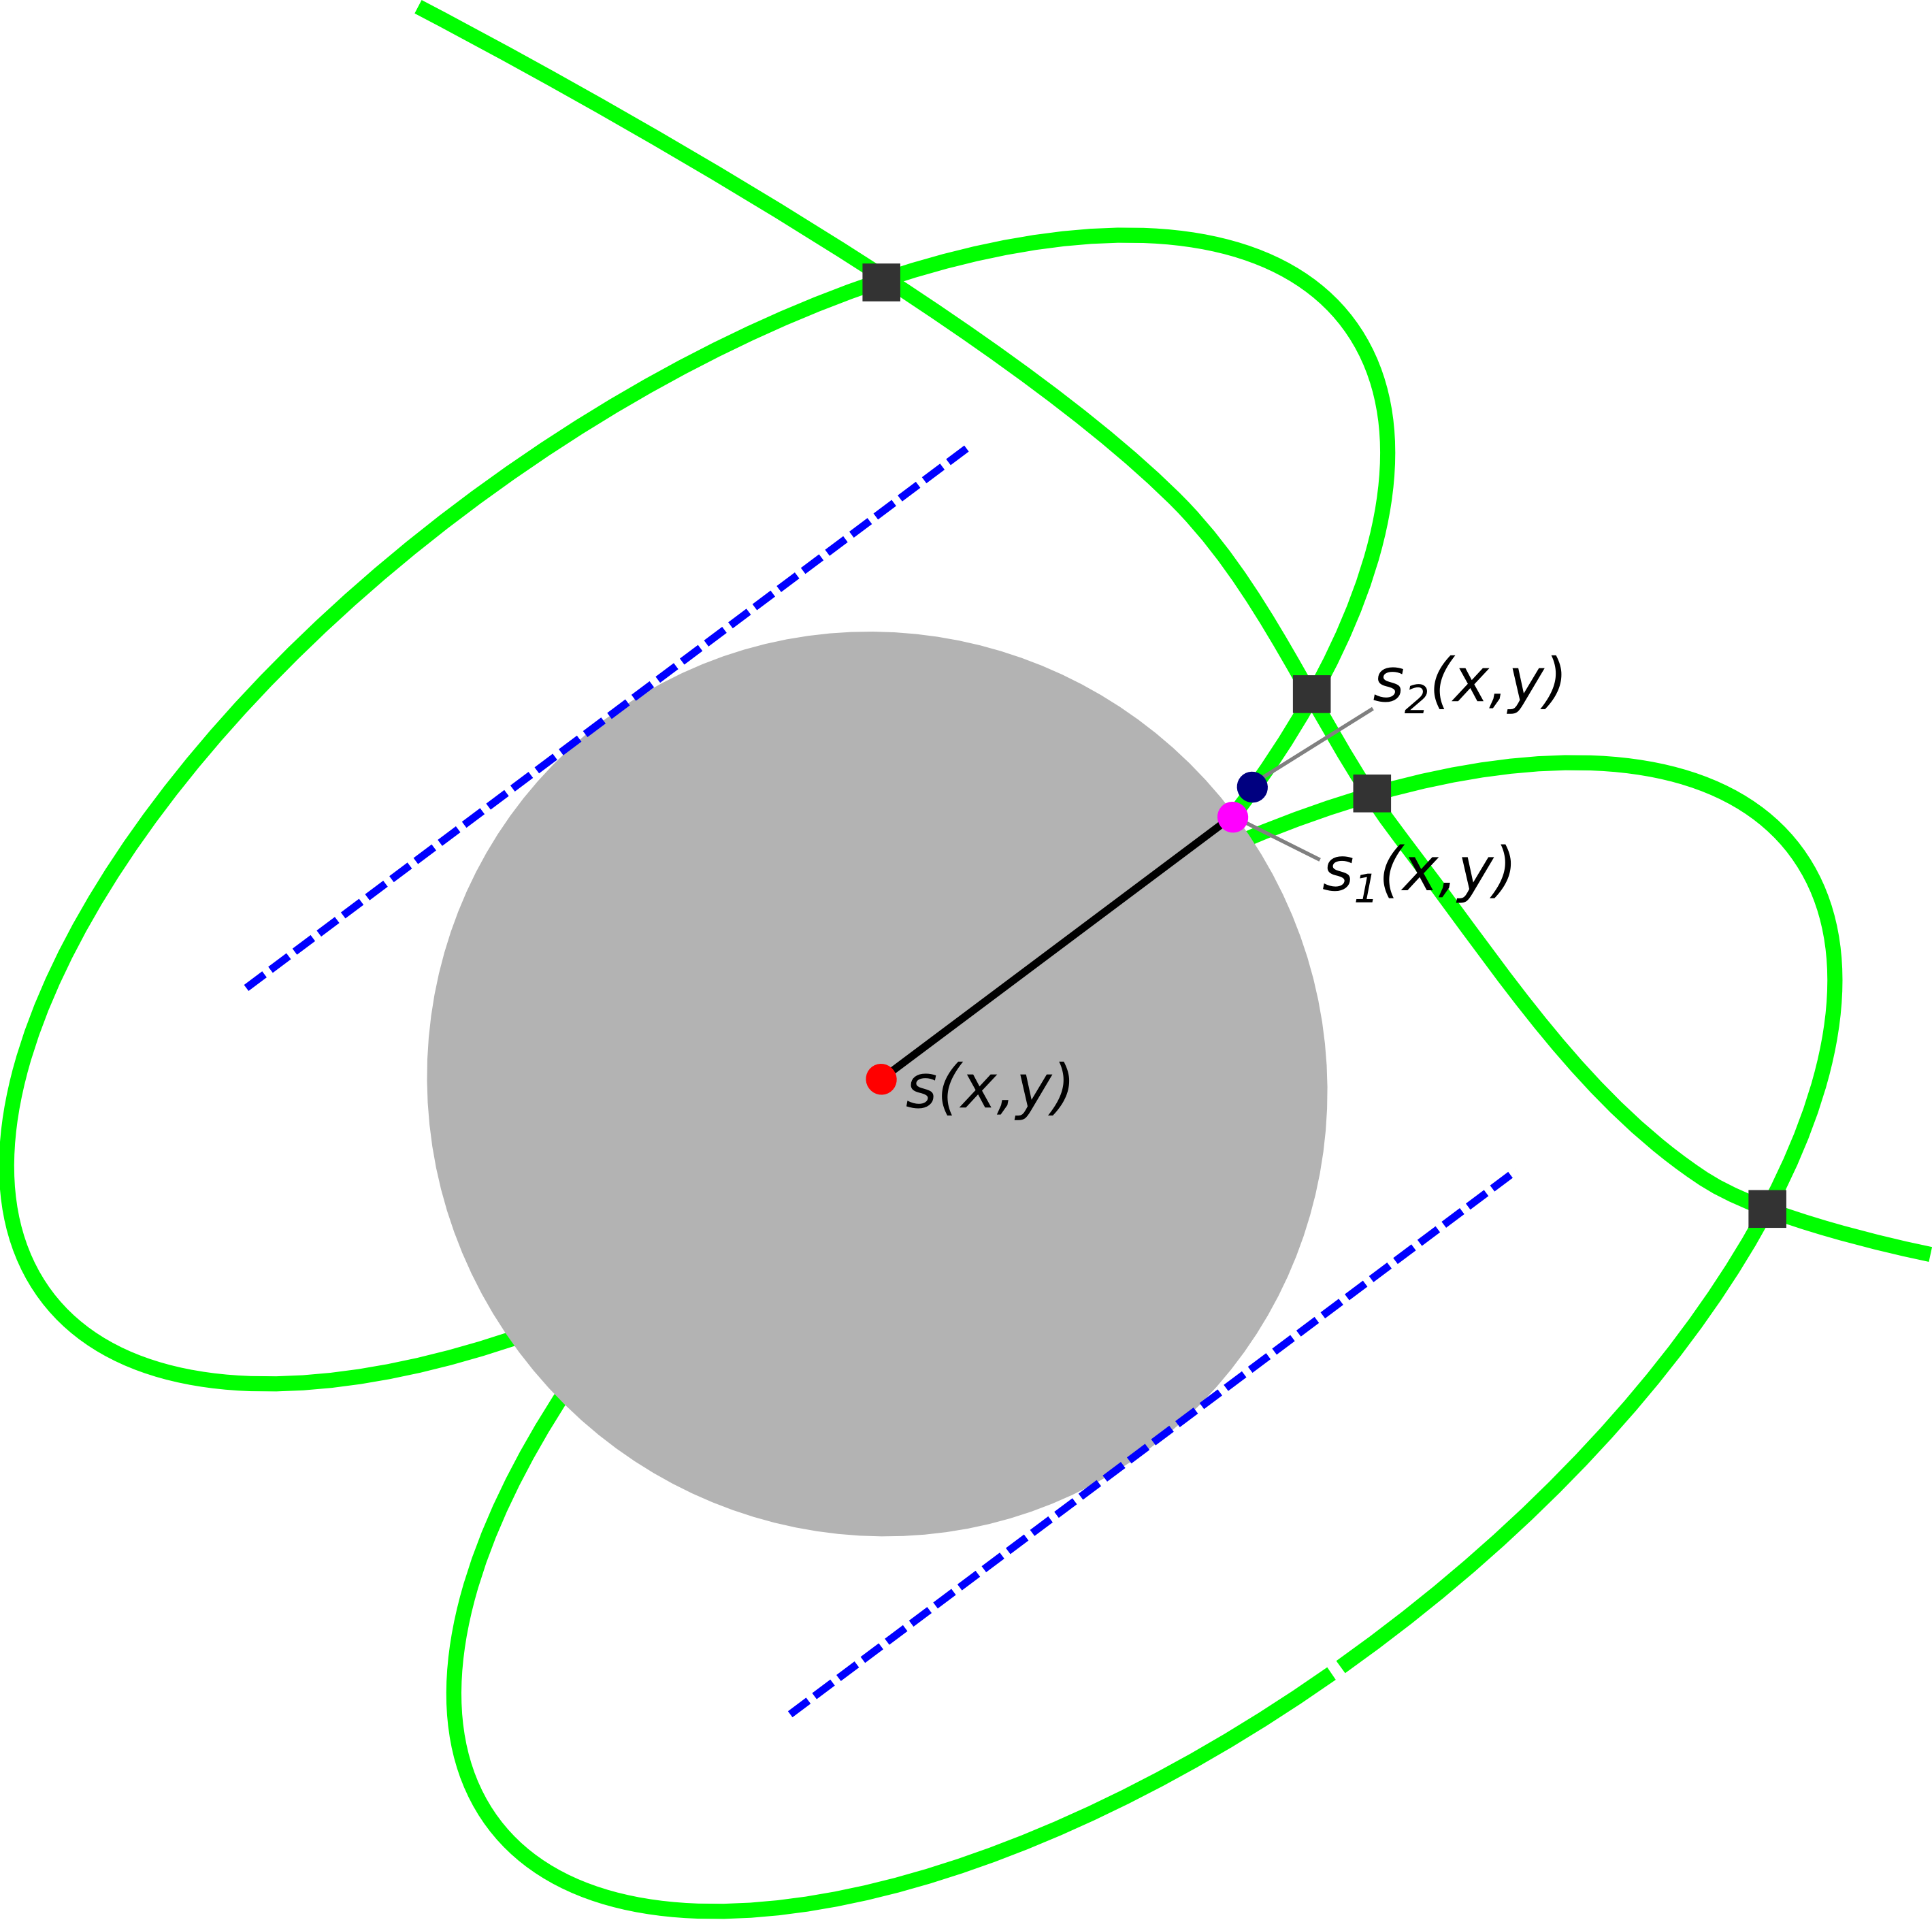
\includegraphics[height=0.4\textheight]{figure6}
% 	    \end{figure}
% 	  \end{block}
% 	}
% 	\only<5-> {
% 	  \begin{block}{Shortest path calculation}
% 	    \begin{itemize}
% 	      \item Connectivity between $s_2$ and $g_2$ is checked.
% 	      \item Dijkstra is applied and the path obtained.
% 	    \end{itemize}
% 	  \end{block}
% 	}
%       }
%       
%     \end{overlayarea}
%   \end{columns}
% 
%   \note{
%   \begin{itemize}
%     \item Footprint generation
%   \end{itemize}
% 
%   }
% \end{frame}

\begin{frame}{Global planning}
 \begin{figure}
  \includemovie[autoplay, repeat, controls]{\textwidth}{0.8\textheight}{/home/nestor/Seafile/Videos/Tesis/cp06/MSVM.mp4}
 \end{figure}
\end{frame}
